\documentclass[
    11pt, % The default document font size, options: 10pt, 11pt, 12pt
%codirector, % Uncomment to add a codirector to the title page
]{charter}


% El títulos de la memoria, se usa en la carátula y se puede usar el cualquier lugar del documento con el comando \ttitle
\titulo{Predicción de series de tiempos aplicado al trading de criptomonedas usando la arquitectura de Transformers}

% Nombre del posgrado, se usa en la carátula y se puede usar el cualquier lugar del documento con el comando \degreename
%\posgrado{Carrera de Especialización en Sistemas Embebidos}
%\posgrado{Carrera de Especialización en Internet de las Cosas} 
\posgrado{Carrera de Especialización en Inteligencia Artificial}
%\posgrado{Maestría en Sistemas Embebidos} 
%\posgrado{Maestría en Internet de las cosas}

% Tu nombre, se puede usar el cualquier lugar del documento con el comando \authorname
% IMPORTANTE: no omitir titulaciones ni tildación en los nombres, también se recomienda escribir los nombres completos (tal cual los tienen en su documento)
\autor{Ing. Martín Leonardo Centurión}

% El nombre del director y co-director, se puede usar el cualquier lugar del documento con el comando \supname y \cosupname y \pertesupname y \pertecosupname
\director{director a definir}
\pertenenciaDirector{pertenencia}
\codirector{} % para que aparezca en la portada se debe descomentar la opción codirector en los parámetros de documentclass
\pertenenciaCoDirector{FIUBA}

% Nombre del cliente, quien va a aprobar los resultados del proyecto, se puede usar con el comando \clientename y \empclientename
\cliente{Nombre del cliente}
\empresaCliente{Empresa del cliente}

\fechaINICIO{15 de octubre de 2024}        %Fecha de inicio de la cursada de GdP \fechaInicioName
\fechaFINALPlan{03 de diciembre de 2024}    %Fecha de final de cursada de GdP
\fechaFINALTrabajo{febrero de 2026}    %Fecha de defensa pública del trabajo final

\begin{document}

    \maketitle
    \thispagestyle{empty}
    \pagebreak


    \thispagestyle{empty}
    {\setlength{\parskip}{0pt}
    \tableofcontents{}
    }
    \pagebreak


    \section*{Registros de cambios}
    \label{sec:registro}


    \begin{table}[ht]
        \label{tab:registro}
        \centering
        \begin{tabularx}{\linewidth}{@{}|c|X|c|@{}}
            \hline
            \rowcolor[HTML]{C0C0C0}
            Revisión & \multicolumn{1}{c|}{\cellcolor[HTML]{C0C0C0}Detalles de los cambios realizados} & Fecha      \\ \hline
            0        & Creación del documento                                                          & \fechaInicioName \\ \hline
            1      & Se completa hasta el punto 5 inclusive                & 30 de octubre de 2024 \\ \hline
            2      & Se completa hasta el punto 9 inclusive                & 4 de noviembre de 2024 \\ \hline
            3      & Se completa hasta el punto 12 inclusive                & 11 de noviembre de 2024 \\ \hline
            4      & Se completa hasta el punto 15 inclusive                & 18 de noviembre de 2024 \\ \hline
%2      & Se completa hasta el punto 9 inclusive
%		  Se puede agregar algo más \newline
%		  En distintas líneas \newline
%		  Así                                                    & {día} de {mes} de 202X \\ \hline
%3      & Se completa hasta el punto 12 inclusive                & {día} de {mes} de 202X \\ \hline
%4      & Se completa el plan	                                 & {día} de {mes} de 202X \\ \hline

% Si hay más correcciones pasada la versión 4 también se deben especificar acá

        \end{tabularx}
    \end{table}

    \pagebreak



    \section*{Acta de constitución del proyecto}
    \label{sec:acta}

    \begin{flushright}
        Buenos Aires, \fechaInicioName
    \end{flushright}

    \vspace{2cm}

    Por medio de la presente se acuerda con \authorname\hspace{1px} que su Trabajo Final de la \degreename\hspace{1px}
    se titulará ``\ttitle'' y consistirá en la implementación de un sistema de predicción de series de tiempos
    aplicado al trading de criptomonedas usando la arquitectura de Transformers.
    El trabajo tendrá un presupuesto preliminar estimado de 614
    horas y un costo estimado de \$44.131.250, con fecha de inicio el \fechaInicioName\hspace{1px}
    y fecha de presentación pública en \fechaFinalName.

    Se adjunta a esta acta la planificación inicial.

    \vfill

% Esta parte se construye sola con la información que hayan cargado en el preámbulo del documento y no debe modificarla
    \begin{table}[ht]
        \centering
        \begin{tabular}{ccc}
            \begin{tabular}[c]{@{}c@{}}
                Dr. Ing. Ariel Lutenberg \\ Director posgrado FIUBA
            \end{tabular} & \hspace{2cm} &
            \begin{tabular}[c]{@{}c@{}}
                \clientename \\ \empclientename
            \end{tabular} \vspace{2.5cm} \\
            \multicolumn{3}{c}{\begin{tabular}[c]{@{}c@{}}
                                   \supname \\ Director del Trabajo Final
            \end{tabular}} \vspace{2.5cm} \\
        \end{tabular}
    \end{table}


    \section{1. Descripción técnica-conceptual del proyecto a realizar}
    \label{sec:descripcion}
    Este es un proyecto personal con el objetivo de estudiar, en el contexto de análisis y predicción de series de tiempo,
    el desempeño de la arquitectura de Transformers. Esta tecnología es una pieza fundacional del estado del arte actual
    en deep learning en general y en predicción de series de tiempos en particular.

    Para dicho estudio se propone la aplicación a un sistema de trading de criptomonedas con el que se espera obtener
    rendimiento y, al mismo tiempo, regular el nivel de riesgo incurrido.

    Es valioso explorar el uso de Transformers y sus variantes, ya que permitiría obtener una ventaja comparativa con
    respecto a otras soluciones mediante la utilización de nuevos modelos basados que presenten mejor poder de predicción.

    El objetivo del trading consiste en obtener una ganancia al comprar instrumentos, en este caso criptomonedas, a un precio menor al que se los vende.
    Se caracteriza por tener un plazo de tiempo acotado, ya que en el largo plazo las fluctuaciones del mercado pierden relevancia
    frente a las condiciones fundamentales del instrumento en cuestión.
    Esto es: el precio del bitcoin (BTC) de hoy a diez años depende más de tendencias macroeconómicas que de otras fluctuaciones.
    Al otro extremo está el trading de alta frecuencia donde se realizan varias operaciones por segundo y requiere del uso de hardware y redes especializadas.
    Por lo expuesto se decide acotar el plazo de predicción entre un minuto y una semana.

    El resultado final, como ilustra la figura \ref{fig:diagBloques}, constará de un sistema capaz de comprar y vender criptomonedas de forma autónoma, el que realiza consultas a un modelo preentrenado con datos históricos sobre cotizaciones pertinentes.


    \begin{figure}[htpb]
            \centering
            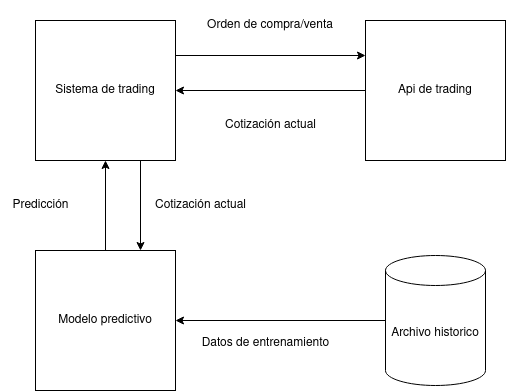
\includegraphics[width=.65\textwidth]{./Figuras/bloques-tp-final.drawio.png}
            \caption{Diagrama en bloques del sistema.}
            \label{fig:diagBloques}
        \end{figure}

    \newpage
    \section{2. Identificación y análisis de los interesados}
    \label{sec:interesados}

    \begin{table}[ht]
        \begin{tabularx}{\linewidth}{@{}|l|X|X|l|@{}}
            \hline
            \rowcolor[HTML]{C0C0C0}
            Rol         & Nombre y Apellido & Organización  & Puesto                     \\ \hline
            Responsable & \authorname       & FIUBA         & Alumno                     \\ \hline
            Orientador  & \supname          & \pertesupname & Director del Trabajo Final \\ \hline
            Cliente  & \authorname          & FIUBA & Alumno \\ \hline
        \end{tabularx}
        \label{tab:interesados}
    \end{table}
    \begin{itemize}
        \item Orientador: \supname.
        \item Responsable: el alumno encargado de llevar a cabo la planificación e implementación.
        \item Potencial cliente: individuo con capital disponible para invertirlo.
    \end{itemize}


    \section{3. Propósito del proyecto}
    \label{sec:proposito}
    El propósito de este proyecto es la investigación y aplicación de arquitecturas de Transformers para el trading de criptomonedas.
    Se buscará explorar esta nueva tecnología y comparar su desempeño con otros modelos previamente utilizados en la industria.


    \section{4. Alcance del proyecto}
    \label{sec:alcance}
    El proyecto incluye:
    \begin{itemize}
        \item El desarrollo de un sistema que realice trading de criptomonedas de forma no supervisada.
        \item Análisis y visualización de los datos históricos correspondientes a las cotizaciones de las criptomonedas seleccionadas.
        \item La exploración de modelos del estado del arte para el análisis y predicción de series de tiempo.
        \item El rango temporal máximo a predecir es de una semana.
        \item El rango temporal mínimo a predecir no implica el uso de hardware especializado ni la conexión a redes especiales.
    \end{itemize}
    El proyecto no incluye:
    \begin{itemize}
        \item Un servicio, ni una API para exponer el modelo.
        \item Aprovisionamiento de infraestructura para correr el modelo.
        \item Implementación de un modelo.
    \end{itemize}


    \section{5. Supuestos del proyecto}
    \label{sec:supuestos}
    Para el desarrollo del presente proyecto se supone que:

    \begin{itemize}
        \item Existen API's con las que integrarse para realizar el trading.
        \item Existen datasets históricos para entrenar los modelos.
        \item La arquitectura de transformers es efectiva para la predicción de series de tiempo.
        \item Existen modelos adecuados para entrenarlos.
        \item Los modelos se pueden entrenar sin hardware especializado.
    \end{itemize}

    \section{6. Requerimientos}
    \label{sec:requerimientos}

    \begin{enumerate}
    \item Requerimientos funcionales:
      \begin{enumerate}
      \item El sistema debe poder operar de forma autónoma.
      \item El usuario debe poder ingresar credenciales de una cuenta en un exchange de criptomonedas con la que operar.
      \item El sistema debe poder detenerse de forma segura.
      \item El sistema debe tener parámetros configurables que determinen el nivel tolerable, para un criterio de riesgo a definir.
      \item Al sistema se le puede definir un monto máximo con el que operar.
      \end{enumerate}
    \item Requerimientos de documentación:
      \begin{enumerate}
      \item Debe estar documentado como iniciar y detener el sistema de forma segura.
      \item Debe estar documentado los parámetros de configuración y como afectan al comportamiento del sistema.

      \end{enumerate}
    \item Requerimiento de testing:
      \begin{enumerate}
      \item El sistema contará con tests de integración contra la API del exchange elegido.
      \item El sistema contará con tests de componente que validen las reglas de negocio del servicio. Por ejemplo: respetar el monto máximo o el limite de riesgo.
      \item El modelo será evaluado según su capacidad predicativa y tendrá en cuenta los datos históricos disponibles.
      \item Se diseñará una forma de monitorizar el rendimiento del sistema.
      \end{enumerate}

    \item Requerimientos de la interfaz:
      \begin{enumerate}
      \item El sistema proveerá una interfaz de línea de comandos (CLI) para iniciar y detener el sistema.
      \item La CLI será clara en sus errores cuando faltase información necesaria para iniciar el sistema.
      \end{enumerate}

    \end{enumerate}

    \section{7. Historias de usuarios (\textit{Product backlog})}
    \subsection{Roles}
    Se identifican los siguientes roles:
    \begin{itemize}
    \item Inversor: individuo registrado en el exchange que aporta la cuenta con capital disponible para operar.
    \item Ingeniero de Operaciones: individuo con conocimientos técnicos responsable de poner el sistema en marcha y velar por su correcto funcionamiento.
    \item Gerente de inversiones: individuo encargado de decidir los parámetros con los que se configurará el sistema con base en los objetivos de negocio.
    \end{itemize}

    \label{sec:backlog}
    \subsection{Product backlog}
    \subsubsection{Inversor}
    \begin{enumerate}
    \item \textbf{Como} inversor \textbf{quiero} proveer de forma secura las credenciales de mi cuenta \textbf{para} que se pueda operar con el capital disponible.
      \textit{Story points}: 3 (complejidad: 1, dificultad: 1, incertidumbre: 1)
    \end{enumerate}

    \subsubsection{Ingeniero de Operaciones}
    \begin{enumerate}
    \item \textbf{Como} ingeniero de operaciones \textbf{quiero} poder levantar el sistema \textbf{para} corroborar que no haya errores de configuración.
      \textit{Story points}: 3  (complejidad: 1, dificultad: 1, incertidumbre: 1)
    \item \textbf{Como} ingeniero de operaciones \textbf{quiero} poder iniciar el sistema \textbf{para} que empiece a operar.
      \textit{Story points}: 8  (complejidad: 2, dificultad: 2, incertidumbre: 3)
    \item \textbf{Como} ingeniero de operaciones \textbf{quiero} poder detener el sistema \textbf{para} que deje de operar.
      \textit{Story points}: 3  (complejidad: 1, dificultad: 1, incertidumbre: 1)
    \item \textbf{Como} ingeniero de operaciones \textbf{quiero} poder detener el sistema de forma segura \textbf{para} que no queden transacciones sin finalizar.
      \textit{Story points}: 5  (complejidad: 3, dificultad: 1, incertidumbre: 1)
    \item \textbf{Como} ingeniero de operaciones \textbf{quiero} poder matar el sistema \textbf{para} que deje consumir recursos.
      \textit{Story points}: 1  (complejidad: 1, dificultad: 1, incertidumbre: 1)
    \item \textbf{Como} ingeniero de operaciones \textbf{quiero} ver logs del sistema  \textbf{para} monitorizar errores.
      \textit{Story points}: 1  (complejidad: 1, dificultad: 1, incertidumbre: 1)
    \end{enumerate}


    \subsubsection{Gerente de inversiones}
    \begin{enumerate}
    \item \textbf{Como} gerente de inversiones  \textbf{quiero} configurar el nivel de riesgo \textbf{para} evitar la perdida de capital.
      \textit{Story points}: 8  (complejidad: 1, dificultad: 2, incertidumbre: 3)
    \item \textbf{Como} gerente de inversiones \textbf{quiero} configurar un límite de dinero a invertir \textbf{para} evitar la perdida de capital.
      \textit{Story points}: 5  (complejidad: 1, dificultad: 2, incertidumbre: 2)
    \end{enumerate}

    \section{8. Entregables principales del proyecto}
    \label{sec:entregables}

    Los entregables del proyecto son:

    \begin{itemize}
    \item Documentación.
    \item Código fuente.
    \item Memoria del trabajo final.
    \item Prototipo funcional a la memoria del trabajo final.
    \item Informe de avance.
    \end{itemize}

    \section{9. Desglose del trabajo en tareas}
    \label{sec:wbs}

    \begin{enumerate}
    \item Estudio del dominio del problema (176 h):
      \begin{enumerate}
      \item Búsqueda de bibliografía (8 h).
      \item Estudio sobre trading (40 h).
      \item Estudio sobre indicadores y análisis técnico (40 h).
      \item Estudio sobre trading algorítmico (30 h).
      \item Estudio sobre análisis de series de tiempo I (24 h).
      \item Estudio sobre análisis de series de tiempo II (24 h).
      \item Estudio sobre compra/venta de criptomonedas (10 h).
      \end{enumerate}

    \item Procuración y análisis de datos (38 h):
      \begin{itemize}
      \item Obtención de datos (3 h).
      \item Análisis y tratamiento (10 h).
      \item Exploración y visualización inicial (15 h).
      \item Entrenamiento y selección de un modelo simple para hacer de base (10 h).
      \end{itemize}

    \item Exploración de métodos tradicionales y estado del arte (150 h):
      \begin{enumerate}
      \item Métodos tradicionales I: moving averages, autoregresión, ARIMA, State Space Models, etc. (25 h).
      \item Métodos tradicionales II: moving averages, autoregresión, ARIMA, State Space Models, etc. (25 h).
      \item Estado del arte I: RNN, CNN, Hybrids, Prophet, DeepAR, etc. (25 h).
      \item Estado del arte II: RNN, CNN, Hybrids, Prophet, DeepAR, etc. (25 h).
      \item Entrenamiento y selección de modelos (30 h).
      \item Visualización y exploración (20 h).
      \end{enumerate}

    \item Exploración del uso de transformers en series de tiempo (100 h):
      \begin{enumerate}
      \item Investigación redes neuronales, transformers, estado del arte, etc. (20 h).
      \item Entrenamiento y selección de modelos (50 h).
      \item Visualización y exploración (20 h).
      \item Comparativa con estado del arte (10 h).
      \end{enumerate}

    \item Implementación del sistema de trading (100 h):
      \begin{enumerate}
      \item Integración con la API del exchange para compra/venta (20 h).
      \item Parametrización de las variables riesgo, monto a operar, etc. (15 h).
      \item Integración con la API del exchange para cotizaciones (15 h).
      \item Implementación de la lógica de decisión de compra/venta (15 h).
      \item Integración con el modelo (10 h).
      \item Productización de la CLI (15 h).
      \item Desarrollo de la lógica de monitorización del rendimiento (20 h).
      \item Documentación (5 h).
      \end{enumerate}

    \item Escritura de las memorias (50 h).
    \end{enumerate}

    Cantidad total de horas: 614.
    \section{10. Diagrama de Activity On Node}
    \label{sec:AoN}


    \begin{figure}[htpb]
      \centering
      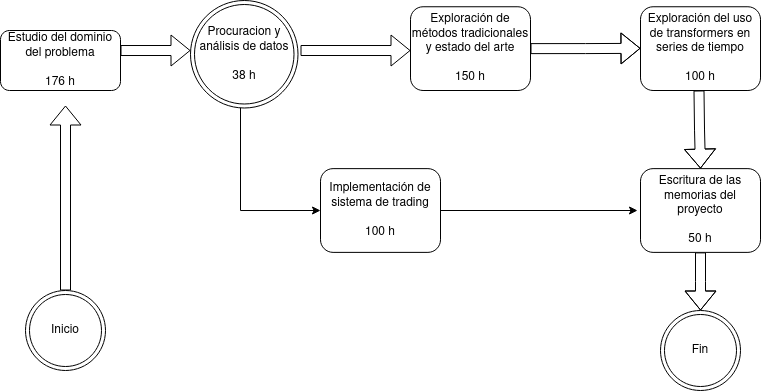
\includegraphics[width=.95\textwidth]{./Figuras/aon.drawio.png}
      \caption{Diagrama de \textit{Activity on Node}. Se ve el camino critico marcado por flechas con volumen. Todas las estimaciones estan en horas. Los hitos están marcados por óvalos.}
      \label{fig:AoN}
    \end{figure}

    \section{11. Diagrama de Gantt}
    \label{sec:gantt}
    \begin{landscape}
      \begin{figure}[htpb]
        \centering
        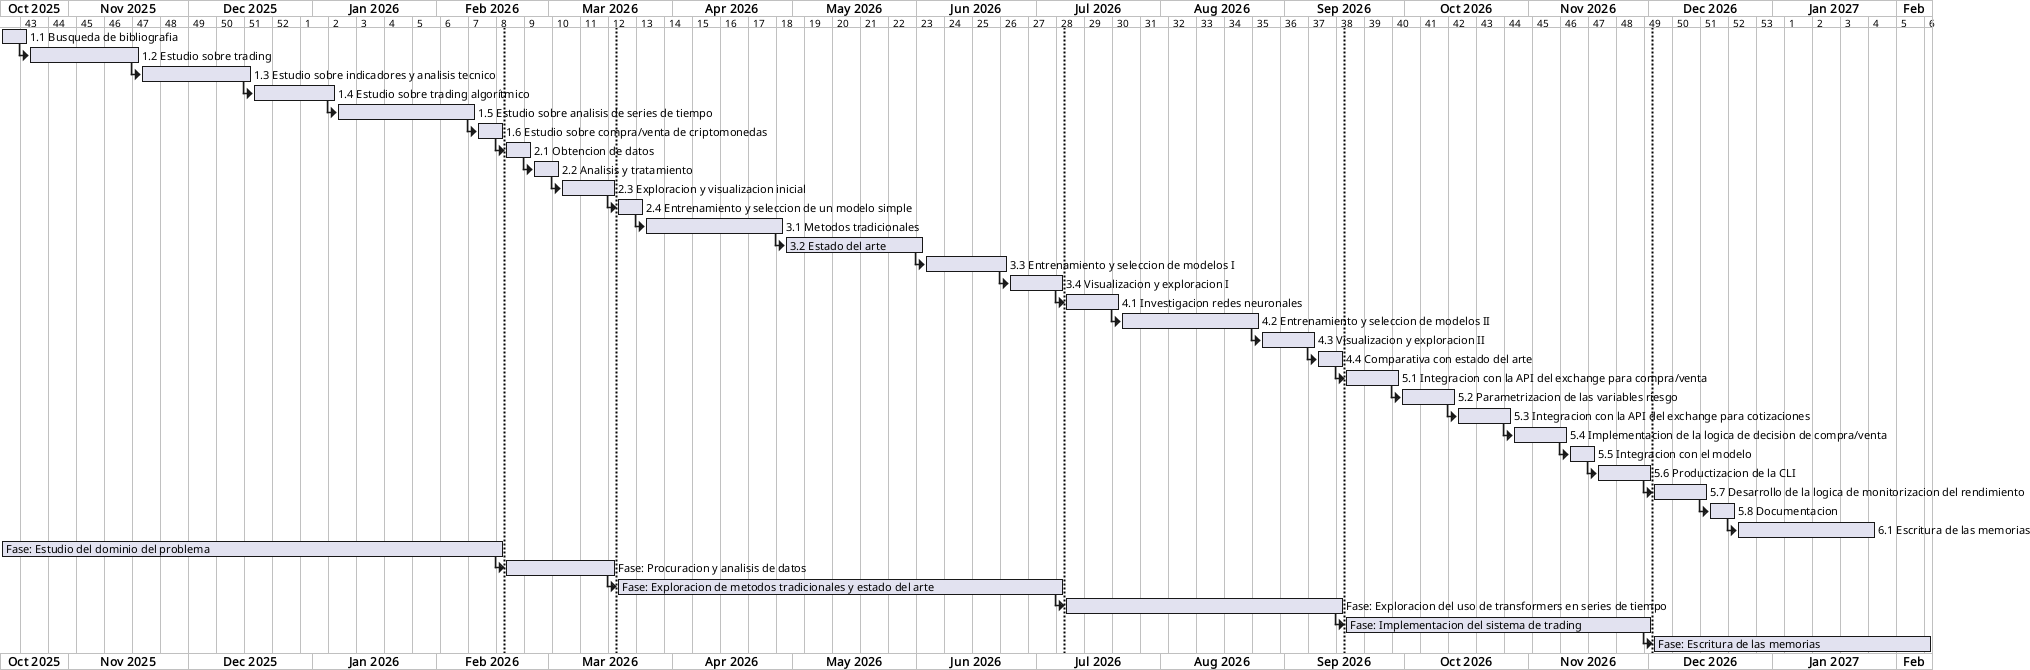
\includegraphics[height=.85\textheight, trim={0 0 40cm 0},clip]{./Figuras/gantt.png}

        \caption{Diagrama de gantt del proyecto (1/2).} %Modificar este título acorde.

        \label{fig:diagGantt1}
      \end{figure}

    \end{landscape}
    \begin{landscape}
      \begin{figure}[htpb]
        \centering
        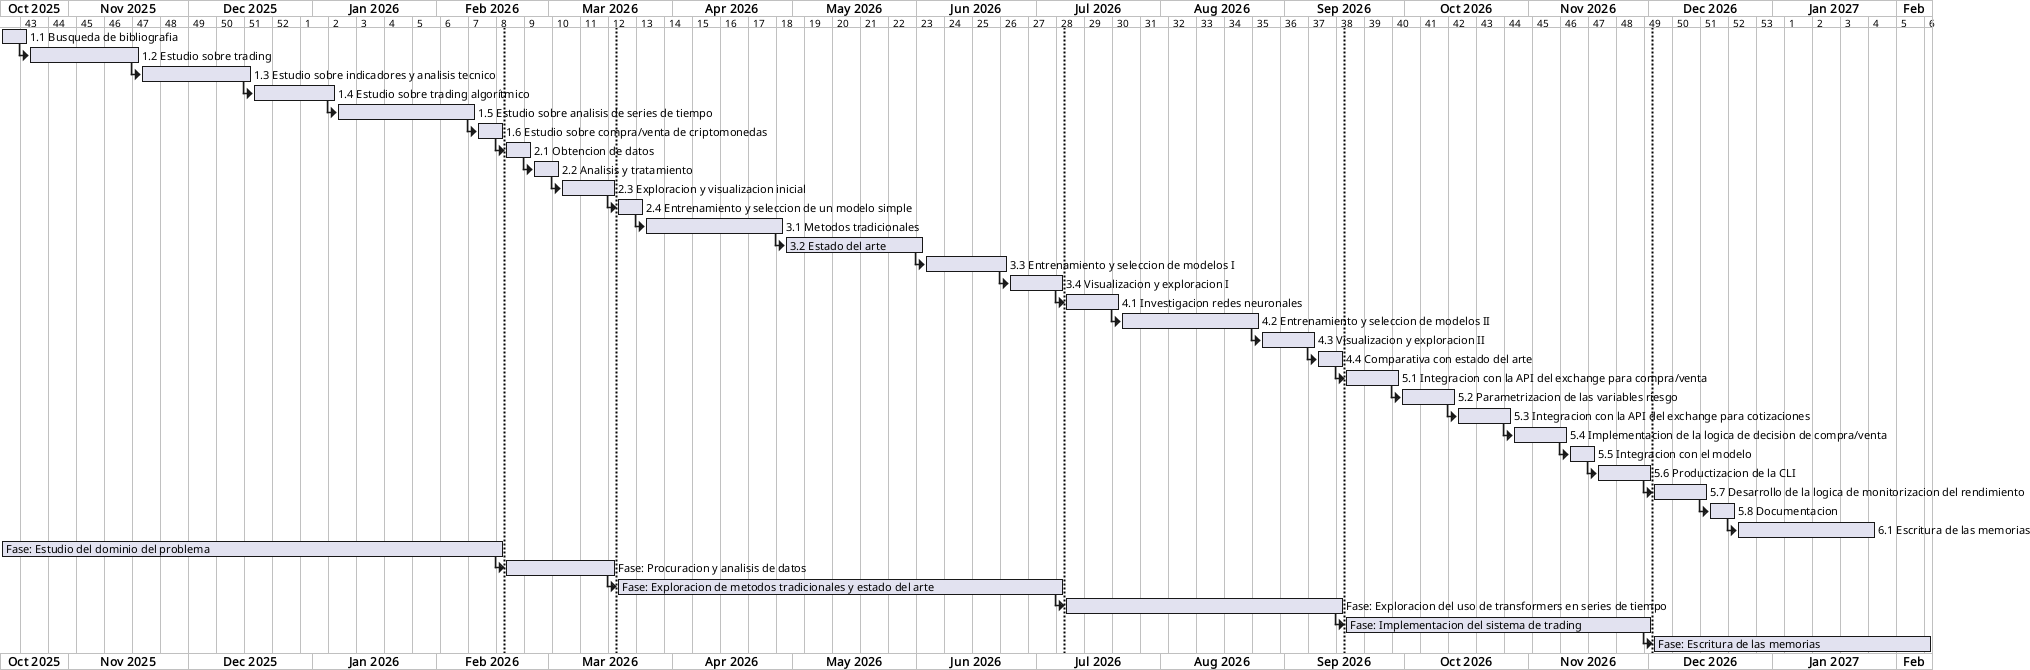
\includegraphics[height=.85\textheight, trim={30cm 0 0 0},clip]{./Figuras/gantt.png}

        \caption{Diagrama de gantt del proyecto (2/2).} %Modificar este título acorde.

        \label{fig:diagGantt2}
      \end{figure}

    \end{landscape}

    \section{12. Presupuesto detallado del proyecto}
    \label{sec:presupuesto}
    \begin{table}[htpb]
        \centering
        \begin{tabularx}{\linewidth}{@{}|X|c|r|r|@{}}
            \hline
            \rowcolor[HTML]{C0C0C0}
            \multicolumn{4}{|c|}{\cellcolor[HTML]{C0C0C0}COSTOS DIRECTOS} \\ \hline
            \rowcolor[HTML]{C0C0C0}
            Descripción &
            \multicolumn{1}{c|}{\cellcolor[HTML]{C0C0C0}Cantidad} &
            \multicolumn{1}{c|}{\cellcolor[HTML]{C0C0C0}Valor unitario} &
            \multicolumn{1}{c|}{\cellcolor[HTML]{C0C0C0}Valor total} \\ \hline
            Horas de trabajo &
            \multicolumn{1}{c|}{614} &
            \multicolumn{1}{c|}{62500 ARS} &
            \multicolumn{1}{c|}{38375000 ARS} \\ \hline

            \multicolumn{3}{|c|}{SUBTOTAL} &
            \multicolumn{1}{c|}{38375000 ARS} \\ \hline
            \rowcolor[HTML]{C0C0C0}
            \multicolumn{4}{|c|}{\cellcolor[HTML]{C0C0C0}COSTOS INDIRECTOS} \\ \hline
            \rowcolor[HTML]{C0C0C0}
            Descripción &
            \multicolumn{1}{c|}{\cellcolor[HTML]{C0C0C0}Cantidad} &
            \multicolumn{1}{c|}{\cellcolor[HTML]{C0C0C0}Valor unitario} &
            \multicolumn{1}{c|}{\cellcolor[HTML]{C0C0C0}Valor total} \\ \hline
            Costos indirectos (15\% de costos fijos) &
            &
            & 5756250 ARS
            \\ \hline
            \multicolumn{3}{|c|}{SUBTOTAL} &
            \multicolumn{1}{c|}{5756250 ARS} \\ \hline
            \rowcolor[HTML]{C0C0C0}
            \multicolumn{3}{|c|}{TOTAL} & 44131250 ARS
            \\ \hline
        \end{tabularx}%
    \end{table}


    \section{13. Gestión de riesgos}
    \label{sec:riesgos}
Riesgo 1: La arquitectura de Transformers no es adecuada para la predicción de series de tiempo en el contexto de las criptomonedas.
        \begin{itemize}
            \item Severidad (S): 10.\\
            La arquitectura de transformers es una pieza central del trabajo.
            \item Ocurrencia (O): 3.\\
            Hay bibliografía disponible que asevere que dicha arquitectura es efectiva para la predicción de series de tiempo.
        \end{itemize}

        Riesgo 2: Se requiere de hardware especializado o de gran poder de cómputo para entrenar los modelos de redes neuronales.
        \begin{itemize}
            \item Severidad (S): 5.\\
            Alquilar o adquirir hardware impactaría en los costos del proyecto.
            \item Ocurrencia (O): 5.\\
            Se desconocen los requerimientos exactos para entrenar los modelos de redes neuronales capaces de predecir series de tiempo de forma efectiva.
        \end{itemize}

        Riesgo 3: La integración, para la lectura de cotizaciones, con la API del exchange es paga.
        \begin{itemize}
        \item Severidad (S): 10.\\
          Limitaría en gran medida el periodo de tiempo con el que se pueden hacer predicciones y la precisión mínima aceptable para estas.
        \item Ocurrencia (O): 1.\\
          Hasta el día de la fecha ha sido gratuita.
        \end{itemize}

        Riesgo 4: La comisión para las transacciones incrementa.
        \begin{itemize}
        \item Severidad (S): 8.\\
          Limitaría la precisión mínima aceptable para las predicciones.
        \item Ocurrencia (O): 3.\\
          Actualmente, para la plataforma Binance, se encuentra en $0.1000\%$. Es una decisión de negocio que depende exclusivamente de la plataforma en cuestión, con lo cual puede cambiar.
        \end{itemize}

        Riesgo 5: Deja de funcionar la computadora con la que se lleva a cabo el desarrollo.
        \begin{itemize}
        \item Severidad (S): 7.\\
          Podría generar perdida de trabajo. Elevaría el costo final del proyecto.
        \item Ocurrencia (O): 2.\\
          No se detectan indicios de falla actualmente.
        \end{itemize}
     \begin{table}[htpb]
            \centering
            \begin{tabularx}{\linewidth}{@{}|X|c|c|c|c|c|c|@{}}
                \hline
                \rowcolor[HTML]{C0C0C0}
                Riesgo & S & O & RPN & S* & O* & RPN* \\ \hline
                Riesgo 1: La arquitectura de Transformers no es adecuada para la predicción de series de tiempo en el contexto de las criptomonedas. & 10  & 3  & 30     &  6  & 3   &    18  \\ \hline
                Riesgo 2: Se requiere de hardware especializado o de gran poder de computo para entrenar los modelos de redes neuronales. & 5  & 5  &  25   &  5  & 5   & 25     \\ \hline
                Riesgo 3: La integración, para la lectura de cotizaciones, con la API del exchange es arancelada.  & 10  & 1  &  10   &    &    &      \\ \hline
                Riesgo 4: La comisión para las transacciones incrementa. & 8  & 3  &  24   &    &    &      \\ \hline
                Riesgo 5: Deja de funcionar la computadora con la que se lleva a cabo el desarrollo. & 7  & 2  &  14   &    &    &      \\ \hline
            \end{tabularx}%
        \end{table}

     Se tomarán medidas de mitigación en los riesgos cuyos números de RPN sean mayores o iguales a 25.


        Riesgo 1: La arquitectura de Transformers no es adecuada para la predicción de series de tiempo en el contexto de las criptomonedas.
        \begin{itemize}
        \item Severidad (S*): 6.
          Existen otros modelos ya sea de deep learning o estadísticos que pueden servir para cumplir el objetivo de predecir el valor del BTC. Estos se exploran en una etapa previa del proyecto.
        \item Probabilidad de ocurrencia (O*): 3.
          La probabilidad no cambia.
        \end{itemize}

        Riesgo 2: Se requiere de hardware especializado o de gran poder de cómputo para entrenar los modelos de redes neuronales.
        \begin{itemize}
        \item Severidad (S*): 5.
          No se mitiga. En caso de ser necesario se contratara un servicio cloud.
        \item Probabilidad de ocurrencia (O*): 5.
          La probabilidad no cambia.
        \end{itemize}

    \newpage
    \section{14. Gestión de la calidad}
    \label{sec:calidad}
    \begin{enumerate}
    \item \textbf{Precisión en las Predicciones:} El modelo debe ser capaz de predecir con alta precisión las fluctuaciones de precios de las criptomonedas (específicamente para un plazo entre un minuto y una semana).
      \begin{itemize}
      \item \textbf{Acción de Verificación:} Realizar pruebas de precisión del modelo que utilice métricas como MAE (Error Absoluto Medio), RMSE (Raíz del Error Cuadrático Medio) y MAPE (Error Porcentual Absoluto Medio) en un conjunto de datos de validación.
      \item \textbf{Acción de Validación:} Comparar las predicciones con un conjunto de datos de test independiente para asegurar que la precisión general es robusta y consistente en diferentes intervalos de tiempo.
      \end{itemize}

    \item \textbf{Eficiencia Computacional:} El modelo debe ser eficiente en términos de tiempo de entrenamiento y capacidad de hacer predicciones en tiempo real.
      \begin{itemize}
      \item \textbf{Acción de Verificación:} Medir los tiempos de entrenamiento y tiempos de inferencia para asegurar que se cumplan los requisitos de tiempo de ejecución. Esto puede incluir la medición del tiempo necesario para entrenar el modelo y hacer una predicción de una nueva entrada de datos.
      \item \textbf{Acción de Validación:} Validar que el sistema puede hacer predicciones en tiempo real dentro de un plazo de menos de un segundo, según las especificaciones del sistema de trading.
      \end{itemize}

    \item \textbf{Robustez ante Ruido de Datos:} El modelo debe ser capaz de manejar el ruido de datos y las fluctuaciones inesperadas del mercado sin perder rendimiento significativo.
      \begin{itemize}
      \item \textbf{Acción de Verificación:} Introducir ruido artificial en los datos de entrada y evaluar la capacidad del modelo para mantener una precisión razonable en la predicción.
      \item \textbf{Acción de Validación:} Evaluar el rendimiento del modelo con datos históricos que incluyan fluctuaciones y eventos inesperados en el mercado, como crisis o “flash crashes”.
      \end{itemize}

    \item \textbf{Modelado de Tendencias a Largo Plazo:} El modelo debe ser capaz de captar tendencias a largo plazo, más allá de las fluctuaciones de corto plazo, como en un plazo de predicción de una semana.
      \begin{itemize}
      \item \textbf{Acción de Verificación:} Utilizar métricas de predicción de largo plazo, como la capacidad del modelo para capturar correctamente las tendencias (por ejemplo, con el coeficiente de determinación R² o una métrica de tendencia direccional).
      \item \textbf{Acción de Validación:} Validar que el modelo puede predecir correctamente las tendencias de criptomonedas de hasta una semana.
      \end{itemize}

    \item \textbf{Minimización del Riesgo:} El sistema debe ser capaz de gestionar y regular el nivel de riesgo asociado a las inversiones.
      \begin{itemize}
      \item \textbf{Acción de Verificación:} Implementar un algoritmo de gestión de riesgo que incluya criterios como stop-loss, take-profit y asignación de capital basada en el riesgo calculado.
      \item \textbf{Acción de Validación:} Validar el modelo con backtesting para evaluar cómo se comporta en diferentes condiciones del mercado, y asegurar que el riesgo no excede los límites establecidos.
      \end{itemize}

    \item \textbf{Redacción de una memoria final:} Se debe redactar una memoria técnica sobre lo que se realizó a lo largo del proyecto.
      \begin{itemize}
      \item \textbf{Acción de Verificación:} tener el documento escrito.
      \item \textbf{Acción de Validación:} publicar el documento.
      \end{itemize}

    \item \textbf{Generación de Señales de Trading Efectivas:} El modelo debe generar señales de compra y venta con un umbral de efectividad aceptable según un indicador de rendimiento como el Sharpe Ratio o el Ratio de Ganancia/Perdida.
      \begin{itemize}
      \item \textbf{Acción de Verificación:} Evaluar la efectividad de las señales generadas al comparar las señales de trading con los movimientos de mercado reales.
      \item \textbf{Acción de Validación:} Validar que las señales generadas por el sistema en condiciones de mercado normales y extremas tengan un impacto positivo en las ganancias netas durante el backtesting.
      \end{itemize}

    \item \textbf{Sistema autonomo:} El sistema debe ser totalmente autónomo en la compra y venta de criptomonedas.
      \begin{itemize}
      \item \textbf{Acción de Verificación:} realizar pruebas con el sistema en funcionamiento por más de un día.
      \item \textbf{Acción de Validación:} realizar pruebas con el sistema en funcionamiento por más de un día.
      \end{itemize}

    \item \textbf{Reportes de transacciones:} El modelo deberá tener alguna forma de exportar las transacciones que se realizaron.
      \begin{itemize}
      \item \textbf{Acción de Verificación:} emitir registro de las transacciones a medida que se realizan.
      \item \textbf{Acción de Validación:} mostrar el registro de las transacciones al cliente.
      \end{itemize}

    \item \textbf{Detención segura del sistema:} el sistema debe poder detenerse de forma segura.
      \begin{itemize}
      \item \textbf{Acción de Verificación:} Probar el mecanismo de detención para asegurarse que no queden transacciones pendientes.
      \item \textbf{Acción de Validación:} Mostrar que, al detener el sistema, no quedan transacciones pendientes.
      \end{itemize}

    \end{enumerate}

    \section{15. Procesos de cierre}
    \label{sec:cierre}
    \begin{itemize}
    \item Pautas de trabajo que se seguirán para analizar si se respetó el Plan de Proyecto original:\\

      \begin{itemize}
      \item Responsable: \supname
      \item Procedimiento: se evaluará el cumplimiento de los requerimientos en tiempo y forma. De no ser el caso se desarrollaran las causas y mitigaciones para futuros proyectos.
      \end{itemize}

    \item Identificación de las técnicas y procedimientos útiles e inútiles que se emplearon, los problemas que surgieron y cómo se solucionaron:\\
      \begin{itemize}
      \item Responsable: \supname
      \item Procedimiento: se evaluarán si las técnicas y procedimientos propuestos fueron efectivos para cumplir con los objetivos. Si se utilizaron otras técnicas y procedimientos que no fueron propuestos también se detallaran.
      \end{itemize}

    \item Indicar quién organizará el acto de agradecimiento a todos los interesados, y en especial al equipo de trabajo y colaboradores:\\
      \begin{itemize}
      \item Responsable: \supname
      \item Procedimiento: presentación final ante las autoridades del CEIA.
      \end{itemize}

    \end{itemize}
\end{document}

% LocalWords:  State Space
